\documentclass[11pt]{article}
\usepackage{amsmath}
\usepackage{amssymb}
\usepackage{array}
\usepackage{graphicx}
\graphicspath{{tests/}{./}}

% --- Manual page geometry (no geometry.sty dependency) ---
\setlength{\textwidth}{6.5in}
\setlength{\textheight}{9.0in}
\setlength{\oddsidemargin}{0in}
\setlength{\evensidemargin}{0in}
\setlength{\topmargin}{-0.5in}
\setlength{\headheight}{0in}
\setlength{\headsep}{0in}
\setlength{\parindent}{0pt}
\setlength{\parskip}{6pt}
\renewcommand{\arraystretch}{1.25}

\begin{document}

% ============ TITLE BLOCK ============
\begin{center}
{\LARGE\bfseries GOWC: An Open Tool for Observing-Conditions}\\[3pt]
{\LARGE\bfseries Prediction and Observation Planning,}\\[3pt]
{\LARGE\bfseries Validated Against Site Monitors and an ETC}\\[12pt]
{\large Ahzam Ahmed}\\[4pt]
{\normalsize Independent researcher \quad$\cdot$\quad ORCID 0009-0007-3864-0934}\\[2pt]
{\normalsize \texttt{ahzamahd641@gmail.com}}\\[2pt]
{\normalsize Global Observing-conditions Weather Catalogue (GOWC)}\\[2pt]
{\small \texttt{gowcastroclimate.com} \quad$\cdot$\quad September 2026}
\end{center}

\vspace{8pt}

% ============ ABSTRACT ============
\begin{center}
\begin{minipage}{0.9\textwidth}
{\small
\textbf{Abstract.} GOWC (Global Observing-conditions Weather Catalogue) is an open web
application that takes the user from a target to an exposure plan across $2{,}642$
catalogued observatory sites, computing seeing, airmass, extinction, precipitable
water vapour, sky brightness and signal-to-noise from live Open-Meteo meteorology
including pressure-level profiles, and validating each output against independent
references. The photometric SNR calculator reproduces the ING \textsc{signal}
exposure-time calculator to a median $2.0\%$ across a magnitude--airmass grid on two
instruments. Seeing is computed from the Tatarski $C_n^2$ chain with a per-level
integration over the pressure levels above the site, calibrated at Paranal via a
MASS/DIMM decomposition; hindcast against $\sim$20 months of ESO Astronomical Site
Monitor DIMM data it shows a real night-to-night ranking skill --- Spearman
$\rho=+0.36$ ($N=588$ nights) at Paranal and $+0.31$ at La Silla,
surviving deseasonalising. Benchmarked candidly, persistence (last night's measured
seeing) scores higher, but GOWC adds independent information beyond it (partial
$\rho=+0.29$) and does so at the $\sim$2{,}600 sites that have no monitor at all.
Model precipitable water vapour is
validated against the Paranal LHATPRO radiometer ($\rho=+0.95$, 606 nights; the
comparison also exposed and fixed a column-altitude double-counting bug, after which
the absolute scale carries a $+40\%$ wet bias).
Throughout, GOWC distinguishes measurement-backed outputs from indicative ones, and
displays the real measured value wherever a public site monitor exists. It is a
planning aid, not a substitute for on-site measurement.

\vspace{4pt}
\noindent\textbf{Keywords:} atmospheric effects --- site testing --- methods:
observational --- techniques: photometric --- astronomical instrumentation ---
software: public release.
}
\end{minipage}
\end{center}

\vspace{6pt}

% ============ 1. INTRODUCTION ============
\section{Introduction}

Planning a night at an optical telescope involves several steps. The observer
first confirms that the target reaches a usable altitude during astronomical
darkness, then estimates the conditions for that night (seeing, transparency, and
sky brightness with the Moon up), and finally sets an exposure time for the
required precision. Each step depends on the one before it, but the tools do not:
visibility comes from planetarium software, conditions from a weather page or
forecast, and signal-to-noise from an instrument-specific exposure-time
calculator (ETC).

GOWC (Global Observing-conditions Weather Catalogue) combines this workflow in one open web
application covering $2{,}642$ catalogued observatory sites. Its design
priority is that every reported number can be traced to a published physical
model with stated assumptions, with no hidden fit. This paper describes those
models, validates them against site monitors and a professional ETC, and states
where the method breaks down. The results are intended for ranking observing nights
at a site, order-of-magnitude exposure times, and absolute quantities flagged with
their uncertainty wherever the input data cannot support more.

This paper makes four contributions. First, it sets out a complete, reproducible
forward planning chain --- visibility, seeing, extinction, precipitable water vapour,
sky brightness and photometric SNR --- driven by one shared physics module across a
catalogue of $2{,}642$ sites rather than a single facility. Second, it benchmarks the
SNR path against a professional exposure-time calculator across a magnitude--airmass
grid, agreeing to a median $2.0\%$ on two instruments. Third, it quantifies the seeing
model's night-to-night ranking skill over a 20-month hindcast against the ESO
Astronomical Site Monitor, and measures it against the baselines an observer already
has --- persistence and surface wind --- reporting the partial correlation that
survives both. Fourth, it states quantity by quantity which outputs are
measurement-backed, which are calibrated, and which are passed through unvalidated.

% ============ 2. SYSTEM OVERVIEW ============
\section{System Overview}

GOWC is a full-stack application. The observatory list is built from the IAU
Minor Planet Center observatory-code list (retrieved 2026-08-31; with several
flagship research facilities added by hand), giving $2{,}642$ catalogued sites. The
MPC codes include many small and amateur stations, so this is a count of catalogued
observatory sites rather than of major professional facilities. Site elevations are taken
from a digital-elevation lookup at each site's coordinates; for a small fraction
($\sim$9\,\%, those whose MPC coordinates round to a whole degree or lack a
sub-arcminute position) the elevation --- and hence the altitude-dependent seeing
and extinction --- is unreliable, and those sites are flagged rather than trusted. A scheduled job fetches weather for every
observatory from Open-Meteo: surface fields (cloud, humidity, wind, temperature,
pressure, precipitation) and pressure-level profiles --- temperature, geopotential
height and wind at 850, 700, 600 and 500\,hPa, wind at 250\,hPa (the jet stream), and
relative humidity at 850 and 500\,hPa --- plus the model total-column water vapour. A shared physics module reads these from a database and converts
them into observing quantities, which two front-ends serve: an interactive
dashboard and a REST API. A guided planning
workflow runs on top of the physics engine. It handles target and site selection,
computes visibility and the best window, applies the night's conditions, solves
for exposure and SNR, and produces an exportable observing plan.

\begin{figure}[t]
\centering
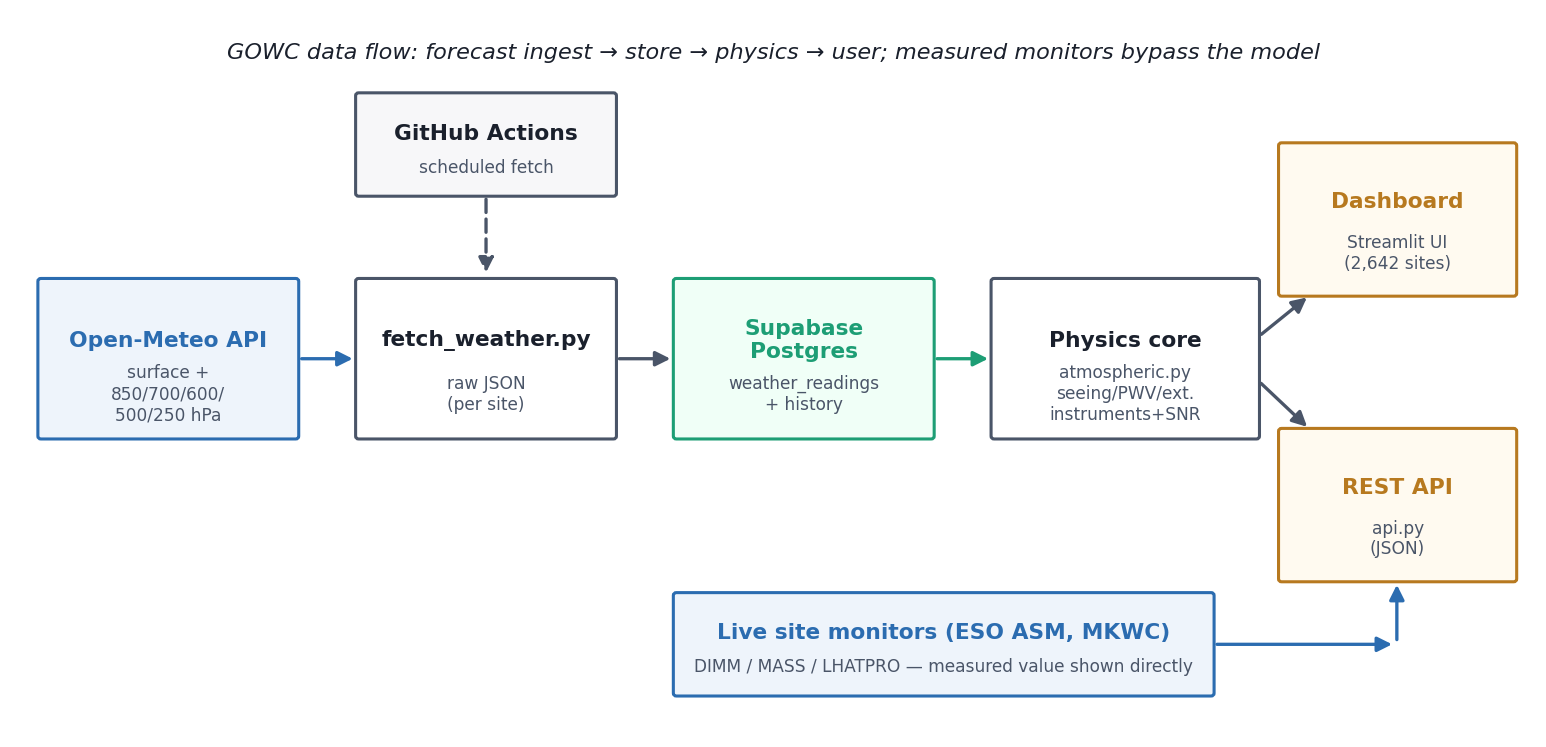
\includegraphics[width=\textwidth]{fig_arch.png}
\caption{GOWC data flow. A scheduled GitHub Actions job pulls surface and
pressure-level fields from Open-Meteo through \texttt{fetch\_weather.py} into a
Supabase Postgres store; a shared physics core (\texttt{atmospheric.py} plus the
instrument/SNR catalogue) converts them into observing quantities, served by an
interactive Streamlit dashboard and a REST API. Where a public site monitor exists
(ESO ASM DIMM/MASS/LHATPRO, Maunakea Weather Center) its \emph{measured} value is
shown directly, bypassing the forecast model.}
\label{fig:arch}
\end{figure}

\paragraph{Scope: the forward half of the pipeline.} The standard photometric
workflow has two halves. The \emph{forward} (predictive) half turns a target
magnitude into expected detector counts and a signal-to-noise ratio, through the
chain flux $\to$ magnitude $\to$ atmospheric extinction $\to$ collected photons
$\to$ SNR. The \emph{reverse} (reduction) half recovers a calibrated magnitude
from a real frame: centroiding and PSF fitting, aperture and annulus sky
estimation, relative photometry against comparison stars, and zero-point
calibration against standard stars. GOWC implements the forward half in full ---
including the Vega/UBVRI system, the Bouguer extinction law (with the secondary,
colour-dependent term $k = k_1 + k_2(B\!-\!V)$ reported alongside the result), and the
instrumental-to-standard colour term --- and predicts the magnitude uncertainty
$\sigma_m = 1.0857/\mathrm{SNR}$ that the reverse half would ultimately measure.
It does not perform the reduction steps, because it never handles a real image;
those follow standard procedures at the telescope and are outside its scope.

\paragraph{Provided tools.} Beyond the core physics, GOWC exposes a set of
observer-facing tools, all driven by the same engine and live data. For
planning: a live weather map of all sites, object-visibility and observing-window
calculators, site comparison, a guided ``Plan an Observation'' wizard, and the
SNR/exposure calculator. For analysis: atmospheric analysis (seeing, extinction,
jet stream, PWV), historical reliability, and telescope efficiency. For transient
and event work: a Transient Follow-Up tab that lists active neutron-star X-ray
binaries with live outburst alerts from the MAXI monitor (this first version
covers X-ray binaries; other classes are flagged as forthcoming), and a Sky
Events section with trackers for meteor showers, eclipses, comets, satellite
passes, and near-Earth asteroids (the latter drawn live from NASA's NeoWs/NEO
service). A literature-search tool queries the NASA ADS database, and an
observing assistant answers plain-language planning questions using the
deterministic engine rather than invented numbers. Registered users can save
sites and log sessions.

\paragraph{Relation to existing tools.} The individual computations GOWC performs
are available elsewhere, but in separate tools: target visibility and airmass in
Astroplan \cite{astroplan}; sky brightness, extinction and exposure times in the
ESO exposure-time calculators and \textsc{skycalc} \cite{skycalc}; instrument-specific
SNR in per-facility calculators such as ING \textsc{signal} \cite{signal}. What GOWC adds is their \emph{combination} in one place
--- visibility, live atmospheric conditions (seeing, PWV, extinction, sky
brightness) and photometric SNR, computed from one shared physics module --- across
a global catalogue of $\sim$2{,}600 sites rather than a single facility, and with
each output traceable to a published model and, where possible, validated against a
site monitor. It is the breadth (many sites, the whole planning chain) rather than
the depth at any one facility that distinguishes it.

\paragraph{Installation, usage and reproducibility.} GOWC runs as a hosted web
application (\texttt{gowcastroclimate.com}); the physics engine is a standalone
Python package (dependencies: \texttt{numpy}, \texttt{pandas}, \texttt{astropy},
\texttt{ephem}, \texttt{requests}) installable from the repository with \texttt{pip install .}\ and
usable without the web layer. The core entry points are direct function calls --- for
example
\begin{quote}\small\texttt{rank\_sites(ra\_deg, dec\_deg, date\_utc)}\end{quote}
returns the candidate observatories ranked by tonight's observability (airmass,
dark-time window and moonlit sky) for a target, and
\texttt{get\_full\_atmospheric\_analysis(record)} returns the seeing, PWV and
jet-stream diagnostics for a site from its weather record. The repository ships the
re-runnable scripts that reproduce every number in Tables~1--6 and the three data
figures (Figures~2--4; Figure~1 is a schematic)
(\texttt{tests/}: \texttt{validate\_\allowbreak snr\_\allowbreak etc.py}, \texttt{snr\_\allowbreak grid\_\allowbreak compare.py},
\texttt{dimm\_\allowbreak mass\_\allowbreak decomposition.py},
\texttt{hindcast\_\allowbreak multiyear.py} with its baseline correlations,
\texttt{hindcast\_\allowbreak extras.py} for the partial correlations, per-year and
out-of-window splits and poor-night skill,
\texttt{validate\_\allowbreak pwv\_\allowbreak lhatpro.py}, and
\texttt{make\_\allowbreak paper\_\allowbreak figures.py} /
\texttt{make\_\allowbreak arch\_\allowbreak figure.py} for the figures), alongside unit-style
validation scripts for the airmass and extinction primitives against their reference
values (\texttt{tests/validate\_airmass.py}, \texttt{tests/validate\_extinction.py}). The scheduled
weather ingest and precompute run under GitHub Actions (twice-daily fetch and a daily
precompute); the validation scripts above are stand-alone and re-runnable, and wiring
them into the same Actions workflow as a regression check is a small, planned step.
This paper
describes GOWC v1.0 (MIT-licensed); the exact version is archived at the Zenodo DOI
in \S7.

% ============ 3. METHODS ============
\section{Physical Models}

All quantities below are computed from the cited formalism. Constants are quoted
as implemented.

\subsection{Seeing}
Seeing (FWHM, arcsec) is derived from the Tatarski $C_n^2$ formulation
\cite{tatarski} driven by real vertical temperature gradients from the pressure
levels above the site (850/700/600/500\,hPa; see \emph{Free-atmosphere
integration} below), following the modern re-derivation of Basu \& Holtslag
\cite{basu}. With potential temperature $\theta = T(1000/P)^{R/c_p}$:
\[
\Gamma = \frac{d\theta}{dz},\quad
C_T^2 = \frac{c}{\mathrm{Pr}_t}L_0^{4/3}\Big(\tfrac{T}{\theta}\Big)^{2}\Gamma^2,\quad
C_n^2 = \Big(\tfrac{79\times10^{-6}P}{T^2}\Big)^{2}C_T^2,
\]
\[
r_0 = \big(0.423\,k^2 X\!\int\! C_n^2\,dh\big)^{-3/5},\qquad
\varepsilon = 0.98\,\lambda/r_0,
\]
with $k=2\pi/\lambda$, the Fried parameter $r_0$ \cite{fried} referenced at
$\lambda=500$\,nm, $\mathrm{Pr}_t$ the turbulent Prandtl number, and seeing FWHM
written as $\varepsilon$ (the potential temperature is $\theta$). To make the implementation reproducible, the remaining
parameters are stated explicitly:

\emph{Airmass.} The airmass $X$ appears \emph{inside} the $C_n^2$ integral
bracket (slant-path convention), i.e.\ the turbulence integral is scaled by $X$
before the $-3/5$ power, rather than computing a zenith $r_0$ and scaling
afterwards.

\emph{Structure-constant coefficient.} The Tatarski coefficient $c$ multiplies
$C_T^2$, and the per-level scale $C$ (below, \emph{Free-atmosphere integration})
multiplies the $C_n^2$ integral in which $C_T^2$ sits, so the two are exactly
degenerate: only the product $c_{\text{eff}}=c\,C$ is identifiable. We therefore fix
$c=2.8$ (a canonical mid-range value) and calibrate $C$, and report the physically
meaningful quantity $c_{\text{eff}}$. Tatarski's coefficient is quoted across
$2.1$--$3.2$ in the literature; the Paranal-calibrated value $c_{\text{eff}}=2.8
\times0.77=2.16$ lands at the bottom edge of that range --- a consistency check the
calibration passes rather than a fit of unexplained origin. $\mathrm{Pr}_t=1$
applies to the stable nighttime stratification assumed here.

\emph{Potential- to actual-temperature conversion.} The $d\theta/dz$
mixing-length argument yields $C_\theta^2$, the structure constant of
\emph{potential} temperature, but the optical conversion $\partial n/\partial T =
-79\times10^{-6}P/T^2$ acts on \emph{actual}-temperature fluctuations, related by
$T' = (T/\theta)\theta'$. Hence $C_T^2 = (T/\theta)^2 C_\theta^2$
\cite{basu}. At mid-layer $(T/\theta)^2 \approx 0.78$, a $\sim$14\% reduction in
seeing; it is altitude-dependent ($(T/\theta)^2 = 0.91$ at 850\,hPa, $0.67$ at
500\,hPa) so it cannot be absorbed into $\Delta h$. We evaluate it with the
layer-mean $T$ and $\theta$.

\emph{Outer scale.} The turbulence outer scale enters $C_T^2$ as $L_0^{4/3}$, and
we take it directly from the Dewan et al.\ (1993) tropospheric model
\cite{dewan}, the standard in NWP-derived optical-turbulence work
\cite{trinquet}:
\[
L_0^{4/3} = 0.1^{4/3}\times 10^{\,1.64 + 42\,S},
\]
with wind shear $S$ (s$^{-1}$). The form is dimensionally correct and returns
$L_0^{4/3}$ --- exactly the quantity $C_T^2$ requires --- so no separate length
bound on $L_0$ is needed. Two guards are applied in the implementation: the shear
entering the exponent is capped at $S=0.02$\,s$^{-1}$ (the strong-shear end of
Dewan's fit), so a spurious model wind difference cannot inflate $L_0^{4/3}$
without limit, and where no shear is available a representative
$S=3\times10^{-3}$\,s$^{-1}$ is used. Dewan's fit takes the \emph{local} shear, so in the per-level
integration $S$ is the shear across each individual layer (700$\to$600, 600$\to$500,
etc.), matching the layer over which its $\Gamma$ is formed; the two-level fallback
uses the 850$\to$500 shear. Because the shear sits in an exponent
($L_0^{4/3}\propto10^{42S}$), the seeing is sharply sensitive to it:
$\partial(\ln\varepsilon)/\partial S \approx 58$\,s, so a shear error of
$0.001$\,s$^{-1}$ is a $\sim$6\% seeing error --- a robustness figure worth stating,
since forecast wind fields are themselves uncertain at this level. A residual caveat
remains even per-level: a difference across a model layer still under-resolves the
thin-layer shear the Dewan radiosonde
fit was built on.\footnote{The Dewan form replaced an earlier
$L_0=\tfrac12 S/N^2$ (with $N$ the Brunt--V\"ais\"al\"a frequency), which is
dimensionally a timescale, not a length.}

\emph{Free-atmosphere integration.} GOWC integrates $C_n^2$ over the real pressure
levels that lie \emph{above} the site --- 850, 700, 600 and 500\,hPa (250\,hPa
supplies only the jet-stream wind and is not part of the integral) ---
forming $\Gamma$, the Dewan $L_0$ and $C_n^2$ for each adjacent layer and weighting
by that layer's own geometric depth, with the lowest bracket interpolated to the
telescope elevation. Levels below the site are excluded, which removes the
sub-site-slab and marine-inversion contamination that afflicts high sites
(\S\ref{sec:dimm-inv}). A single dimensionless constant $C$ scales the
resulting integral so the free-atmosphere seeing reproduces the measured MASS median
at Paranal ($0.43''$, over the same dates the MASS data span; \S\ref{sec:dimm}),
giving $C=0.77$ --- degenerate with the Tatarski coefficient $c$, so the identifiable
quantity is $c_{\text{eff}}=c\,C=2.16$, checked against the literature range above.
The same constant serves the live Forecast API and the Historical Forecast API used
for the 20-month validation: at matched dates the two products give essentially the
same free-atmosphere seeing ($0.43''$ vs $0.41''$ at Paranal), and their temperature
gradients agree to $\sim$5\%. This per-level scheme replaces an earlier
two-level form in which one 850--500\,hPa gradient stood in for a slab of assumed
thickness $\Delta h$; that $\Delta h$ was a genuine free parameter (calibrated to
$1200$\,m against the same MASS median) and is retained only as a fallback when the
700/600\,hPa levels are unavailable. The per-level scheme carries one calibration
constant in its place, but each layer now has its true geometric depth rather than a
shared assumed one.

One definitional caveat attaches to this lower bound. MASS measures turbulence above
$\sim$500\,m above the site, whereas the integration here begins at the telescope, so
at Paranal the slab from $2635$\,m to the 700\,hPa level ($\sim$3150\,m) sits inside
$\varepsilon_{\text{free}}$ while the DIMM$-$MASS difference of \S4.5 assigns that same
slab to the ground layer. The two terms therefore overlap by roughly one layer.
Numerically this is absorbed into the two calibration constants and nothing downstream
breaks, but it is a mild qualification on two later statements: that
$\varepsilon_{\text{free}}$ reproducing the MASS median is a wholly clean test, and
that the free-atmosphere-vs-DIMM partial correlation ($\rho=+0.29$ after partialling
out \emph{surface wind}; \S4.5) is entirely irreducible to the surface. This is a
different quantity from the full-model partial of $+0.29$ that survives controlling
for \emph{persistence}, also reported in \S4.5.

The pressure levels resolve only the free atmosphere, so the free-atmosphere
value is combined in quadrature with a ground/boundary-layer term (independent
turbulent layers), $\varepsilon_{\text{tot}} = \sqrt{\varepsilon_{\text{free}}^2 +
\varepsilon_{\text{bl}}^2}$; the ground layer dominates real seeing at most
sites (\S\ref{sec:dimm}). Rather than a fixed constant,
$\varepsilon_{\text{bl}}$ is a site-aware surface parametrisation,
\[
\varepsilon_{\text{bl}} = \varepsilon_0\,
\big(1 + (w/8)^2\big)^{0.3}\,
e^{-h/10000}\; X^{0.6},
\]
with surface wind $w$ (m\,s$^{-1}$), site altitude
$h$ (m) and $\varepsilon_0 = 0.77''$ (the numerical coincidence with the
free-atmosphere constant $C=0.77$ above is exactly that --- the two are independent
calibrations, one dimensionless and one in arcseconds): it grows with surface wind
(mechanical shear) and has only a gentle altitude dependence. (An earlier version also carried a
humidity factor $1+\max(0,\mathrm{RH}-40)/150$ as a surface-instability proxy; a
ranking test against DIMM showed it \emph{reduced} skill --- the full-model $\rho$
rose from $+0.34$ to $+0.36$ without it, consistent with humidity's weak link to
optical turbulence --- so it was removed, \S\ref{sec:dimm}.) The scale height is
$10\,000$\,m by design: the ground layer
is a \emph{local} surface phenomenon set by topography and heating, not by
absolute elevation, so even a high site such as Paranal retains a strong ground
layer --- which the MASS/DIMM decomposition of \S\ref{sec:dimm} confirms. The base
$\varepsilon_0$ is calibrated so Paranal at its \emph{median} surface conditions
($w\!\approx\!2.8$\,m\,s$^{-1}$) reproduces the measured
ground-layer median of $0.61''$. Two consequences are stated frankly in
\S\ref{sec:dimm}: with a $10\,000$\,m scale height the ground-layer term is nearly
site-invariant (altitude factor $1.00$ at sea level to $0.64$ at 4500\,m), so most
site-to-site discrimination rests on the free-atmosphere third; and one site cannot
constrain an altitude dependence, so $10\,000$\,m is a chosen, not a fitted, scale
height.
Because seeing varies strongly from night to night, GOWC reports the forecast
value for a given night rather than a site median.

\subsection{Airmass and extinction}
A single airmass definition is used throughout, the Pickering (2002)
interpolative formula \cite{pickering}:
$X = 1/\sin\!\big(a + 244/(165+47a^{1.1})\big)$, $a$ in degrees. Extinction
follows the Bouguer law $\Delta m = k\,X$ with band coefficients anchored to La
Palma monitoring \cite{king} and scaled to site altitude by a single exponential,
$k(h) = k_{\text{ref}}\,e^{-(h - h_{\text{ref}})/H_k}$ with $H_k = 8000$\,m and
$h_{\text{ref}}$ the reference-site altitude; transmission is
$10^{-0.4\,k X}$. This is a deliberate simplification: the Rayleigh component
scales with pressure ($H\approx8400$\,m) while the aerosol component falls far
faster ($H\approx1$--2\,km), so a single scale height cannot represent both
exactly, and the aerosol term (which dominates $k$ at low sites) is the larger
source of residual error. When a target colour is known the secondary
(colour-dependent) term $k = k_1 + k_2(B\!-\!V)$ is reported alongside the result ---
bluer stars are extinguished slightly more per airmass, $k_2$ being largest in the
blue and negligible in the red --- but it is not applied to the single-band $k$ used
in the calculation (Appendix~\ref{app:constants}). The instrumental-to-standard colour term
$m_{\text{std}} = m_{\text{inst}} + \text{zp} + c_t\,(B\!-\!V)$ (with $c_t$ the
colour-term coefficient, distinct from the Tatarski $c$ of \S3.1) is reported
alongside the result.

\subsection{Precipitable water vapour}
PWV uses the data provider's model-computed total-column water vapour --- a
radiative-transfer product, more reliable than deriving PWV from a coarse two-
or three-node humidity profile. The provider integrates the column from the model
grid cell's terrain height $h_{\text{model}}$ (returned with each query), so only
the residual water between that surface and the telescope must be removed: since
water vapour falls roughly exponentially with height,
$\mathrm{PWV}(h_{\text{site}}) = \mathrm{PWV}_{\text{model}}\,
e^{-(h_{\text{site}}-h_{\text{model}})/H_w}$ with scale height $H_w \approx 2000$\,m.
(Scaling from sea level instead, $e^{-h_{\text{site}}/H_w}$, removes the sub-site
column twice; the LHATPRO comparison in \S\ref{sec:pwv} caught this.) A layered
integral of specific humidity from the Magnus relation \cite{magnus} is retained as
a fallback where the column product is unavailable.

\subsection{Sky brightness}
Moonlit sky brightness uses the Krisciunas \& Schaefer (1991) model
\cite{ks1991}, which folds in lunar phase angle, the Moon's and target's
airmasses, and --- the dominant term --- the Moon--target angular separation,
summed against a dark-sky baseline.

\subsection{Signal-to-noise ratio}
The SNR calculator implements the standard CCD equation with scintillation:
\[
\mathrm{SNR} = \frac{S}{\sqrt{S + B_{\mathrm{sky}} + D_c + N_{\mathrm{read}}^2 n_{\mathrm{pix}} + \sigma_{\mathrm{scint}}^2}},
\]
where $S$ is source counts and $B_{\mathrm{sky}}$ and $D_c$ are the sky-background
and dark-current electron totals \emph{summed over} the $n_{\mathrm{pix}}$ pixels of
the aperture (a 1-FWHM radius), so only the read-noise term carries $n_{\mathrm{pix}}$
explicitly; $N_{\mathrm{read}}$ is the per-pixel read noise. The dark-current symbol
$D_c$ is kept distinct from the telescope diameter $D$ in the scintillation term
below and from DIMM seeing $D$ in \S\ref{sec:dimm}. Source flux uses per-band Vega zero-points
\cite{bessell}. Scintillation follows the modern Osborn et al. (2015) form
\cite{osborn}, $\sigma_Y^2 = 10^{-5}C_Y^2 D^{-4/3}t^{-1}X^3 e^{-2h/H}$
($H=8000$\,m, $C_Y\approx1.5$ \cite{kornilov}). Here $\sigma_Y$ is a
\emph{fractional} intensity fluctuation (dimensionless), so it enters the
electron-count noise budget as $\sigma_{\text{scint}} = \sigma_Y\,S$ (i.e.\
$\sigma_{\text{scint}}^2 = \sigma_Y^2 S^2$ in the denominator), scaling with the
source counts $S$; the airmass factor $X^3$ uses the same Pickering airmass as the
rest of GOWC, which departs from $\sec^3 z$ only below $\sim$30$^\circ$ altitude.
Real instrument constants
(aperture, pixel scale, read noise, detector full-well, published zero-point,
and an empirical/theoretical efficiency term) are drawn from a small cited
catalogue of instruments (INT/WFC, WHT/ACAM, pt5m, VLT/FORS2, Keck/LRIS,
Gemini/GMOS). The resulting photometric magnitude uncertainty is reported as
$\sigma_m = 1.0857/\mathrm{SNR}$.

% ============ 4. VALIDATION ============
\section{Validation}

Each quantity is validated against the best available reference: deterministic
quantities against reference tables, and atmospheric quantities against real
instrument measurements where a public site monitor exists.

\subsection{Airmass and extinction}
Airmass is deterministic geometry, so it is checked against the Kasten \& Young
(1989) reference tables \cite{kasten}: GOWC's Pickering (2002) values agree to
better than $0.35\%$ above $5^\circ$ altitude (largest deviation $0.34\%$, at $10^\circ$) (the two forms diverge near the horizon,
reaching $\sim$1.6\% at $0.1^\circ$, well below any realistic observing limit).
Extinction coefficients are \emph{anchored} to
King (1985) at La Palma \cite{king}, so La Palma agreement is by construction; the
altitude-scaled coefficient matches the published Paranal values to
$\le$0.01\,mag/airmass in $BVRI$ ($0.006$ in $V$) and $0.02$ in $U$. We flag, with the same candour applied to PWV
(\S\ref{sec:pwv}), that this is a weak test of the altitude scaling: La Palma
($2400$\,m) to Paranal ($2635$\,m) is a $235$\,m step, over which the scaling factor
moves the coefficient by $<$3\%, so the agreement chiefly re-tests the anchor, and
the extinction scale height itself is essentially unconstrained here.

\subsection{Precipitable water vapour against LHATPRO}
\label{sec:pwv}
GOWC's model column, corrected to the site altitude (\S3.3), is compared to the ESO
LHATPRO radiometer at Paranal over essentially the same 2025--2026 window (nightly
medians, $N=606$ matched nights; the LHATPRO series extends one observing night
earlier than the DIMM baseline, to 2024-12-31, because the local-night binning
assigns the first UTC hours of 2025-01-01 to the preceding observing night). The night-to-night agreement is excellent
--- Spearman $\rho=+0.95$ ($[+0.94,+0.96]$). This validation exposed and fixed a real bug in the altitude
correction: Open-Meteo integrates the total column from the \emph{model grid cell's}
terrain surface (its \texttt{elevation} field, $2617$\,m for the Paranal cell), not
from sea level, so scaling by $e^{-h_{\text{site}}/H_w}$ removed the sub-site water a
second time and biased the column low by a factor $3.7$ relative to the corrected
model column (equivalently $2.7\times$ below the measured LHATPRO median) --- and,
since it worsened with altitude, biased the whole catalogue. Correcting the residual to the model
terrain, $\mathrm{PWV}=\mathrm{PWV}_{\text{model}}\,e^{-(h_{\text{site}}-
h_{\text{model}})/H_w}$, brings the Paranal median to $3.9$\,mm against the measured
$2.8$\,mm --- a $+40\%$ wet bias (relative to the measurement) rather than a factor
of three low. GOWC therefore reports PWV as a validated quantity (ranking
$\rho=0.95$; absolute high by $\sim$40\%), and where the LHATPRO measurement exists
displays it directly. Figure~\ref{fig:pwv} shows the night-to-night agreement: a tight
correlation about a 1:1 line displaced upward by the residual wet bias.

\begin{figure}[!htbp]
\centering
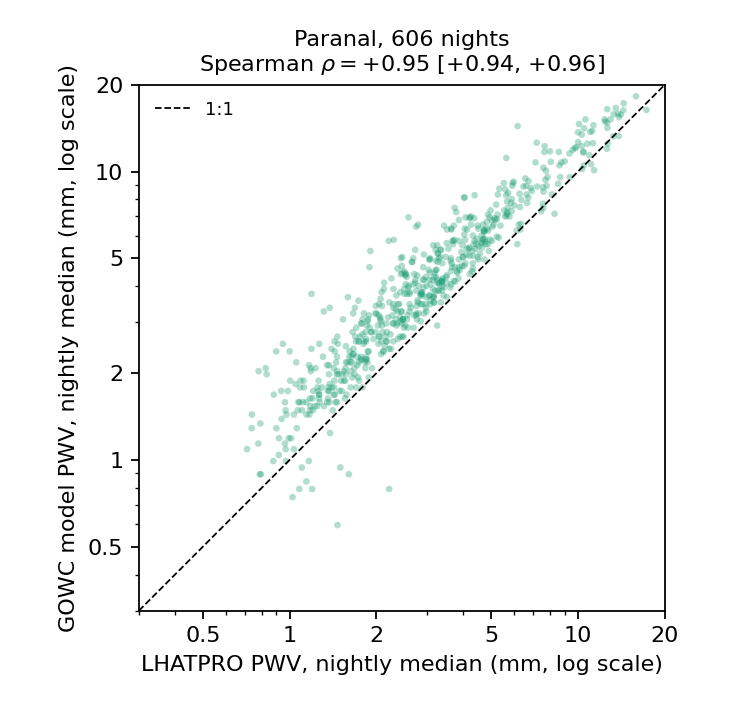
\includegraphics[width=0.62\textwidth]{fig_pwv.png}
\caption{GOWC model-column PWV (corrected to the model-cell terrain, \S3.3) against
the ESO LHATPRO radiometer at Paranal, nightly medians over the 606-night window. The
rank correlation is the strongest in the paper ($\rho=+0.95$); the points sit
consistently above the 1:1 line, the $+40\%$ absolute wet bias of the forecast column
that the altitude correction does not remove.}
\label{fig:pwv}
\end{figure}

Two caveats bound what this test establishes. At Paranal the model cell
($h_{\text{model}}=2617$\,m) sits essentially at the site ($2635$\,m), so the
residual correction factor is $e^{-18/2000}=0.99$ and does nothing: LHATPRO here
validates the \emph{raw} Open-Meteo column and diagnoses the double-count, but says
nothing about the exponential form or the value $H_w=2000$\,m, which remain
unconstrained by any measurement in this work. Yet that exponential is applied
catalogue-wide and does real work at sites whose peak sits well above a coarse grid
cell; testing it needs a site with a large $h_{\text{site}}-h_{\text{model}}$ gap and
a public PWV feed. The residual $+40\%$ wet bias is a property of the forecast
column, not of the correction, and we do not claim to explain it.

\subsection{Cloud cover: passed through, not validated}
Cloud cover is arguably the single most decisive input for whether a night happens
at all, and GOWC fetches it (from Open-Meteo's surface product) and uses it in the
headline observing-quality score. We validate it against no independent reference in
this work: it is passed through as the provider supplies it, and its accuracy is
that of the underlying forecast. A satellite-cloud or all-sky-camera comparison is
the obvious next validation and is not attempted here; the quantity is flagged as
unvalidated wherever it drives a reported score.

\subsection{Signal-to-noise ratio}
We compared the photometric SNR calculator with ING \textsc{signal}, the official
ETC for the Isaac Newton Group telescopes on La Palma, for two instruments. Both
used the same point-source case: $m=20$ in $V$, a 100\,s exposure, $1.0''$
seeing, airmass 1.0, extinction 0.12, dark sky. GOWC matched \textsc{signal}'s
detected counts and SNR to within $\sim$6\% for each (Table~\ref{tab:val}).
To confirm the agreement is not particular to that operating point, we extended the
comparison to a grid in magnitude ($m_V=16$--$22$) and airmass ($X=1.0,1.5$): over
$16$ points the median $|\Delta|$ is $2.0\%$ and every point falls within $6\%$
(median signed ratio $0.999$, i.e.\ no net bias; Appendix~\ref{app:snrgrid},
Table~\ref{tab:snrgrid}).

\begin{table}[h]
\centering
\begin{tabular}{l r r r l}
\hline
\textbf{Instrument} & \textbf{GOWC SNR} & \textbf{\textsc{signal} SNR} & \textbf{ratio} & \textbf{object counts (GOWC/\textsc{signal})} \\
\hline
WHT / ACAM / $V$ & 152.2 & 152.66 & 1.00 & 41{,}675 / 41{,}983 (0.7\%) \\
INT / WFC / $V$  &  92.1 &  89.20 & 1.03 & 15{,}300 / 14{,}425 (6.1\%) \\
\hline
\end{tabular}
\caption{GOWC vs.\ ING \textsc{signal}, identical inputs. A re-runnable
benchmark is provided in the source repository.}
\label{tab:val}
\end{table}

The two instruments failed differently, which made the second test useful. ACAM
agreed at the sub-percent level once the photometry aperture matched
\textsc{signal}'s convention (one-FWHM radius). WFC was initially high by a
constant factor of about 1.4 in both source and sky counts. Because the factor
was the same for source and sky, it had to be a throughput term, and it matched
\textsc{signal}'s ``empirical/theoretical'' efficiency: $\sim$0.70 for WFC
against 1.00 for ACAM, a measured loss below the ideal optical throughput. Adding
it as a per-instrument efficiency removed the discrepancy. The remaining few
percent is consistent with rounding in the zero-points and extinction
coefficient.

\subsection{Seeing: calibration and validation}
\label{sec:dimm}
The seeing model was developed against the ESO Astronomical Site Monitor at
Paranal, which runs both a Differential Image Motion Monitor (DIMM, total seeing)
and a Multi-Aperture Scintillation Sensor (MASS, free-atmosphere seeing above
$\sim$500\,m). Having both on the same timestamps gives two equations for the two
turbulent layers, so the ground-layer contribution follows in quadrature. This is
computed \emph{per timestamp} and then reduced to a median --- medians do not
commute with quadrature subtraction, so $\mathrm{median}\!\sqrt{D^2-M^2} \ne
\sqrt{\mathrm{median}(D)^2-\mathrm{median}(M)^2}$ --- discarding the 0.6\% of
pairs with $M \ge D$ (instrument noise, unphysical). The measured decomposition over
2026-05-29 to 08-29 ($N = 31{,}865$ native-cadence matched pairs) is given in
Table~\ref{tab:decomp}, and the three components are shown as distributions in
Figure~\ref{fig:decomp}.

\begin{table}[h!]
\centering
\begin{tabular}{l r l}
\hline
\textbf{Component (Paranal, measured)} & \textbf{Value} & \textbf{Reduction} \\
\hline
DIMM total seeing              & $0.79''$ & median of $D$ \\
MASS free-atmosphere seeing    & $0.43''$ & median of $M$ \\
Ground layer                   & $0.61''$ & median of $\sqrt{D^2-M^2}$ (per pair) \\
Ground-layer variance fraction & 67\%     & median of $(D^2-M^2)/D^2$ (per pair) \\
ESO's own ground $C_n^2$ fraction & 65\%  & ESO MASS-DIMM product \\
\hline
\end{tabular}
\caption{Measured MASS/DIMM seeing decomposition at
Paranal, each row with its
reduction method. Because the statistics are computed \emph{per timestamp} and then
reduced, the rows are not related by quadrature among their medians (e.g.\ the
ground-layer $0.61''$ is not $\sqrt{0.79^2-0.43^2}$; medians do not commute with
quadrature). The per-pair variance fraction ($67\%$) is corroborated by ESO's
independently-derived ground $C_n^2$ fraction ($65\%$). The window is southern
winter, which in this archive is the \emph{poorer}-seeing part of the year, so these
medians sit above the annual figure (\S\ref{sec:dimm}, Table~\ref{tab:bias}).}
\label{tab:decomp}
\end{table}

\begin{figure}[!htbp]
\centering
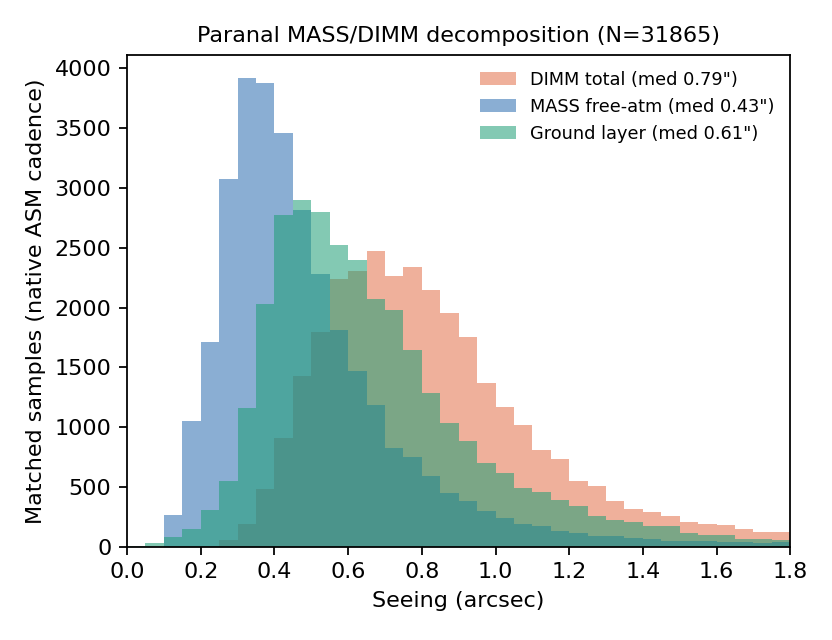
\includegraphics[width=0.72\textwidth]{fig_decomp.png}
\caption{The Paranal MASS/DIMM decomposition as distributions rather than medians.
DIMM total seeing (whole atmosphere), MASS free-atmosphere seeing (above
$\sim$500\,m), and the per-timestamp ground layer $\sqrt{D^2-M^2}$. The ground layer
carries the bulk of the total seeing and its variance; the free-atmosphere third is
the part the model can most cleanly resolve and validate (\S\ref{sec:dimm}).}
\label{fig:decomp}
\end{figure}

\medskip
This decomposition diagnosed a specific, correctable problem. An earlier version
of the model ran $\sim$1.7$\times$ high against DIMM and attributed the bias
wholly to the free atmosphere. The decomposition shows the real picture is two
offsetting errors: the ground layer is \emph{measured} at $0.61''$, but the
earlier parametrisation ($e^{-h/2500}$) suppressed it to $\sim$$0.2''$ at Paranal's
altitude, while the free-atmosphere term was simultaneously too high (a
dimensionally-incorrect outer scale). Correcting the outer scale (Dewan 1993),
relaxing the ground-layer altitude dependence, and adding the $(T/\theta)^2$
structure-constant conversion resolve both.

\paragraph{Calibration (Paranal).} Two constants are \emph{calibrated} to this
site: the free-atmosphere $C_n^2$ integral is scaled so $\varepsilon_{\text{free}}$
matches the measured MASS median ($0.43''$), and the ground-layer base
$\varepsilon_0$ is set so $\varepsilon_{\text{bl}}$ matches the measured
\emph{per-timestamp} ground-layer median ($0.61''$) at Paranal's median surface
conditions. Both terms of $\varepsilon_{\text{tot}}=\sqrt{\varepsilon_{\text{free}}^2
+\varepsilon_{\text{bl}}^2}$ are thereby fixed to measured values at Paranal, so
agreement with the Paranal total is a property of the calibration and carries no
model information. We report it as calibration, full stop; the validating evidence
is the held-out sites and, above all, the ranking hindcast, neither of which enters
the calibration.

\paragraph{Absolute-scale sanity check (other sites).} This is a check on the
absolute \emph{bias} the Paranal calibration produces elsewhere --- not a test of
site ranking, which five sites cannot support (below). GOWC's median seeing (median
of the 20-month nightly hindcast where an ASM archive exists, else a
median-conditions evaluation on the same Historical-Forecast-API fields) is compared
to a measured median at each site in Table~\ref{tab:bias}.

\begin{table}[h!]
\centering
\begin{tabular}{l r r l}
\hline
\textbf{Site} & \textbf{GOWC} & \textbf{Measured} & \textbf{Bias} \\
\hline
Paranal (calibration) & $0.76''$ & $0.75''$ (ASM, this work) & $+1\%$ \\
La Silla              & $0.84''$ & $0.82''$ (ASM, this work) & $+2\%$ \\
La Palma              & $0.84''$ & $0.76''$ (mean) \cite{munoztunon} & $+11\%$ \\
Mauna Kea             & $0.64''$ & $0.6$--$0.7''$ \cite{skidmore} & within range \\
Hanle                 & $0.59''$ & $\sim$$0.9''$ \cite{hanle} & $-34\%$ \\
\hline
\end{tabular}
\caption{Absolute-bias sanity check. GOWC medians for
Paranal and La Silla are the median of nightly medians of the hindcast over
2025--2026 (bootstrap 95\% CI $\pm0.01''$); the others are a single
median-conditions evaluation, all on the Historical-Forecast-API fields with the
free-atmosphere constant $C=0.77$ (\S3.1). The measured Paranal median here
($0.75''$) is lower than Table~2's ($0.79''$) because Table~2 covers the
MASS-matched southern-winter window, which in this archive is the poorer-seeing part
of the year: on this same nightly reduction the May--August nights median $0.80''$
against $0.72''$ for September--April. The change of reduction acts in the opposite
direction and is much smaller (nightly medians run \emph{above} the native-cadence
median, $+0.01''$ over the full baseline), so the seasonal difference alone accounts
for the gap. Measured
medians are the sites' own ASM DIMM archives (Paranal, La Silla) or published
literature; the latter vary with epoch and instrument (published Mauna Kea medians
span $\sim0.46$--$0.68''$ across campaigns; we compare to the $0.6$--$0.7''$
DIMM-based subset, which GOWC's $0.64''$ falls within). The La Palma reference is a
DIMM \emph{mean} rather than a median, so its comparison to GOWC's median is
approximate. This is a
bias/sanity check, \emph{not} a demonstration of site ranking: with $N=5$ the
site-to-site rank correlation is uninformative, and over the four non-calibration
sites a constant $0.76''$ predictor ($10\%$ mean absolute error) about matches the
model ($12\%$, inflated by Hanle; the MAE takes the Mauna Kea reference at the
$0.65''$ midpoint of its DIMM range). Table~3 shows only that the calibrated absolute
scale is in the right regime (three of the four held-out sites within $12\%$; only
Hanle exceeds it); the demonstrated skill is
night-to-night (Table~4), not between sites. Hanle's $-34\%$ is plausibly its
documented strong surface layer, which at 4500\,m the $e^{-h/10000}$ ground-layer
term under-weights (\S5).}
\label{tab:bias}
\end{table}

\medskip

\paragraph{Ranking skill --- measured over 20 months.} Bias and ranking are
independent: a model can be unbiased yet rank at chance, so we test ranking
directly. GOWC's per-level seeing is hindcast through Open-Meteo's Historical
Forecast API --- which archives pressure-level forecast fields from 2021 onward,
distinct from the ERA5 \emph{archive} endpoint (no pressure levels) and the live
forecast API (only $\sim$12 days retained) --- and time-matched to the ESO ASM DIMM
record over 2025-01-01 to 2026-08-28. Both series are on the same geometric footing:
the ASM DIMM reports seeing corrected to zenith, so the model is evaluated at $X=1$
throughout the hindcast and the slant-path factor of \S3.1 plays no part in the
comparison. Because DIMM seeing autocorrelates over 1--3
hours, hourly pairs are not independent; we reduce each site-night to a median (of
the hourly bins available; the correlation is stable under a stricter
$\ge$3-bin-per-night filter, $\rho=+0.35$, $N=584$) and correlate the \emph{nightly}
series, the honest sample. Over the 605-night baseline Paranal supplies 588 usable
nights (97\%) and La Silla 393 (65\%); the difference reflects DIMM availability in
the two ASM archives, not a modelling choice.

Two methodological points frame the result. First, this archive stores each model
run's \emph{initial-hours} fields, i.e.\ near-analysis rather than a multi-day-ahead
forecast; the reported $\rho$ is therefore an \emph{upper bound} on operational
planning skill, and a skill-versus-lead-time curve (Open-Meteo's fixed-offset
previous-run fields do not currently serve pressure levels) is left to future work.
Second, the layer-parameter calibration window (\S\ref{sec:dimm}) lies inside this
baseline. Because the two calibrated constants weight the free-atmosphere and ground
terms independently, their relative value can in principle re-order nights, so we do
not argue the overlap away --- we exclude it: repeating the Paranal correlation on
the $504$ nights \emph{outside} the calibration window (2026-05-29 to 08-29) gives
$\rho=+0.37$ ($[+0.29,+0.44]$), statistically indistinguishable from the full baseline. The ranking skill is
therefore not an artefact of the overlap.

The result is a real, significant positive ranking skill (Table~\ref{tab:multiyear};
the nightly GOWC-vs-DIMM scatter is shown in Figure~\ref{fig:ranking}).

\begin{table}[h!]
\centering
\begin{tabular}{l r r l}
\hline
\textbf{Site (nightly)} & \textbf{$N$ nights} & \textbf{Spearman $\rho$} & \textbf{95\% CI} \\
\hline
Paranal (vs DIMM total)        & 588 & $+0.36$ & $[+0.29,\,+0.43]$ \\
Paranal (vs MASS free-atm.)    &  85 & $+0.36$ & $[+0.16,\,+0.53]$ \\
La Silla (vs DIMM total)       & 393 & $+0.31$ & $[+0.22,\,+0.40]$ \\
\hline
\end{tabular}
\caption{Night-to-night ranking skill of the per-level
model against the ESO ASM, on nightly medians over $\sim$20 months. Confidence
intervals are Fisher-$z$; a moving-block bootstrap gives consistent bounds (Paranal
DIMM $[+0.27,+0.45]$). Paranal is stable across years ($\rho=+0.38$ in 2025 on $N=358$ nights,
$+0.33$ in 2026 on $N=229$); La Silla is more variable ($\rho=+0.43$ in 2025 on $N=209$ nights, $+0.11$
in 2026 on $N=184$), so its full-baseline $+0.31$ is carried mainly by the 2025 half
--- a caution we flag rather than average away. The debiased scatter
--- the RMS of the $\log_{10}$ residuals after removing the median offset --- is
$0.14$\,dex. The model compresses the dynamic range: at Paranal the spread of
$\log_{10}$(model seeing) is $0.40\times$ that of $\log_{10}$(DIMM) ($0.061$ vs
$0.152$\,dex), and an OLS fit of $\log$(model) on $\log$(DIMM) has slope $0.17$ ---
the model orders nights correctly but predicts well under the true spread, which is
why the ranking skill is significant yet modest.
Nightly coverage differs by site --- Paranal $588/605$ nights ($97\%$), La Silla
$393/605$ ($65\%$), reflecting ASM DIMM availability over the baseline --- and the
Paranal correlation is unchanged under a stricter $\ge$3-measurement-per-night filter
($\rho=+0.35$, $N=584$).}
\label{tab:multiyear}
\end{table}

\begin{figure}[!htbp]
\centering
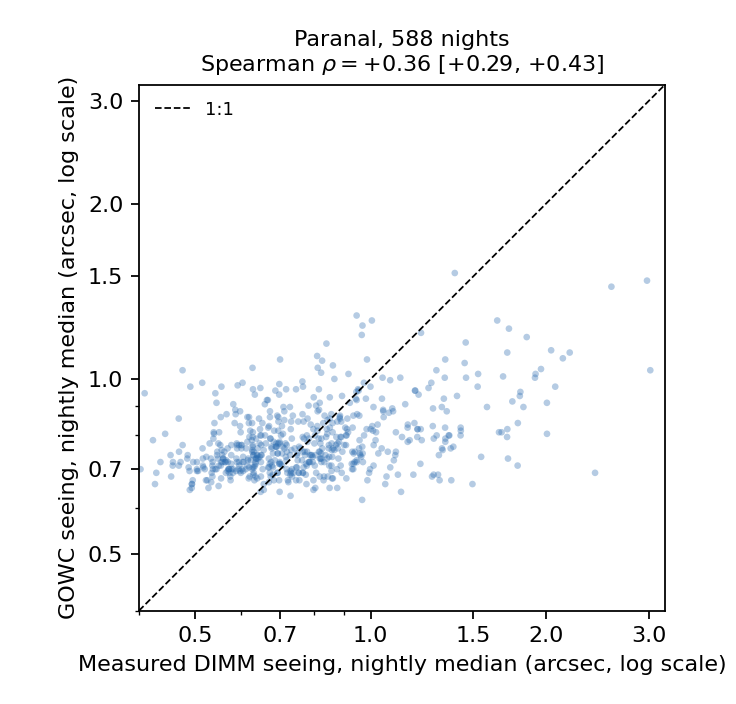
\includegraphics[width=0.62\textwidth]{fig_ranking.png}
\caption{Nightly-median GOWC seeing vs measured DIMM at Paranal over $\sim$20
months. The positive rank correlation is clear, as is the model's compression of the
dynamic range --- it orders nights correctly but under-predicts the spread, which is
why the skill is significant yet modest.}
\label{fig:ranking}
\end{figure}

Every interval excludes zero: the model genuinely orders good and poor nights at a
fixed site.\footnote{An earlier test on a single 12-day window had returned
$\rho\approx-0.4$ from $N=61$ \emph{hourly} pairs; because DIMM seeing autocorrelates
over 1--3 hours those 12 nights amount to only $\sim$2--3 effectively-independent
samples, so the interval spanned zero, and the 20-month baseline supersedes it --- a
reminder that the effective sample size, not the raw pair count, must set the claim,
which is why we report $N$ in \emph{nights} with confidence intervals throughout.}

\emph{Is this seasonal?} Over 20 months both series carry an annual cycle, so part
of $\rho$ could be the model tracking summer-vs-winter rather than
night-to-night. Removing a monthly-climatological median from each series and
re-correlating the anomalies gives $\rho=+0.36$ at Paranal --- unchanged.
The skill is genuinely night-to-night, not a seasonal artefact.

\emph{How does it compare to the predictors an observer already has?} Two cheap
baselines set the bar, and the informative statistic is the \emph{partial}
correlation --- what the model adds beyond each. \emph{Persistence} (last night's
\emph{measured} DIMM median as tonight's forecast) scores $\rho=+0.55$ over 577
consecutive-night pairs, higher than GOWC's $+0.36$ unconditionally; but the partial
correlation of the model with tonight's DIMM, controlling for persistence, is
$\rho=+0.29$ --- so GOWC carries substantial \emph{independent} information beyond
simply repeating last night. \emph{Surface wind alone} (the 10\,m speed) scores
$\rho=+0.33$, close to the full chain; this is expected, since surface wind is itself
an \emph{input} (it drives $\varepsilon_{\text{bl}}$), so it is a component of the
model, not an external competitor. The two terms of the model carry \emph{comparable}
marginal skill --- the ground-layer term $\varepsilon_{\text{bl}}$ scores $\rho=+0.33$
against DIMM total and the free-atmosphere term $\rho=+0.34$ --- so it is not the case
that one dominates the ranking. The distinction appears only in a \emph{partial}
correlation: $\varepsilon_{\text{bl}}$'s skill is essentially its surface-wind input
re-expressed (at a fixed site it varies only through $w$ and the airmass $X$, and
$\rho=+0.33$ is just the wind correlation), whereas the free-atmosphere term retains
$\rho=+0.29$ after partialling out surface wind. So the free-atmosphere Tatarski chain
is \emph{not} decorative --- it contributes independent signal that surface wind does
not --- but the honest statement is that both terms matter and only the free-atmosphere
one is irreducible to the wind. In short, GOWC does not out-score persistence
unconditionally but adds independent skill beyond both persistence and surface wind
(partial $+0.29$ each); \S5 draws out what that means for the unmonitored sites.

\emph{The MASS row is the cleanest test.} The Paranal-vs-MASS correlation
(Table~4, $\rho=+0.36$) is structurally immune to the calibration: $C$ is a purely
multiplicative scale on $\varepsilon_{\text{free}}$ and $\varepsilon_0$ does not
enter $\varepsilon_{\text{free}}$ at all, so no monotonic rescaling can change the
Spearman coefficient. It therefore needs no calibration-window-exclusion argument
(despite its 85 nights lying mostly inside that window), and --- together with the
$\rho=+0.29$ wind-controlled partial above --- it validates the free-atmosphere
physics directly and cleanly.

The skill corresponds to $\rho^2\approx13\%$ of the \emph{rank} variance shared
between model and measurement --- broadly consistent with the $0.14$\,dex debiased
scatter. Cast as the operational question ``will tonight be poor?'' (DIMM
$>1.0''$, a $20\%$ base rate at Paranal), a rate-matched model threshold flags such
nights with a $45\%$ hit rate (recall) at a $14\%$ false-alarm rate. Put as the number an
observer acts on: when the model flags a night as poor it is right $45\%$ of the
time (precision), against the $20\%$ base rate --- more than a twofold enrichment for a site with
no monitor. (Because the threshold is rate-matched, the flag rate equals the base rate,
so precision and recall nearly coincide.) Its magnitude follows from the input resolution. Dedicated mesoscale optical-turbulence forecasts
that resolve the vertical turbulence profile at high resolution (e.g.\ the MOSE /
Astro-Meso-NH system at Paranal \cite{masciadri}) achieve substantially higher
predictive skill, at far greater computational cost and for one site at a time;
GOWC instead drives the published Tatarski chain from five standard pressure levels
across a global catalogue. Its modest skill is therefore expected, and the input
resolution is the named limiting factor rather than the formulation --- a
positioning, not an apology (the physical reason, the coarsely-resolved ground layer,
is set out in \S5). The demonstrated
value of GOWC's seeing is therefore this quantified, modest night-to-night ranking
skill at a fixed site; ranking one site's forecast \emph{seeing} against another's is
not claimed, being neither demonstrated by Table~3 nor expected given the
near-site-invariant ground term (\S5).

This is a narrow disclaimer and should not be mistaken for a wider one. Ranking
\emph{sites} for a given target --- which observatory can observe an object tonight,
for how long, at what airmass, and against what moonlit sky --- rests on airmass and
dark-time geometry, validated to sub-percent (\S4.1), together with the anchored
extinction of \S3.2 and the modelled lunar sky brightness of \S3.4; forecast
seeing enters such a ranking only as a secondary weight, and is superseded by a
measured DIMM value where one is published. What is not claimed is the specific and
much harder statement that the \emph{forecast seeing model alone} orders sites
correctly on a given night.

Independently of the model, where a public site monitor exists GOWC
\emph{displays the measured value directly}: it fetches live DIMM seeing from the
ESO Paranal ASM and the Maunakea Weather Center, and live precipitable-water
vapour from the ESO LHATPRO radiometer at Paranal, falling back to the model
elsewhere. A measurement is ground truth; the model is used only where no
instrument exists.

\subsection{Sky brightness: modelled, not validated here}
\label{sec:skyval}
Moonlit sky brightness (\S3.4) is computed from the Krisciunas \& Schaefer (1991)
model \cite{ks1991}, which remains the standard photometric choice and is well
tested in its original literature. We do not independently validate it in this work:
it is used as published, driving only the dark-time window and the advisory
sky-brightness figure in the exposure planner, never a validated headline output.
A grid comparison against the ESO \textsc{skycalc} sky-radiance model
\cite{skycalc} across lunar phase and Moon--target separation is the natural next
check and is left to future work (\S\ref{sec:future}); the quantity is flagged as
modelled-not-measured wherever it is reported.

% ============ 5. DISCUSSION ============
\section{Discussion and Limitations}

Every model in GOWC is taken from the published literature, with one bespoke piece:
the boundary-layer seeing term $\varepsilon_{\text{bl}}$ (\S3.1) is a calibrated
parametrisation of our own --- its wind and altitude functional form is not drawn
from Dewan or Tatarski --- and we treat it as such throughout. The SNR path is
now backed by a comparison with a professional ETC. GOWC nevertheless runs on
forecast surface and pressure-level data, so it is a planning tool rather than an
instrument pipeline. The outputs therefore separate into two groups.

\emph{On solid ground:} airmass ($<0.35\%$ vs Kasten--Young above $5^\circ$), the Bouguer extinction
form (anchored at La Palma; the Paranal check re-tests the anchor more than the
altitude scaling, \S4.1), the CCD SNR equation (agreement with the \textsc{signal}
ETC to a median $2.0\%$ across a magnitude--airmass grid on two instruments,
Appendix~\ref{app:snrgrid}), and real instrument constants where catalogued.
Precipitable water vapour tracks LHATPRO night-to-night ($\rho=0.95$) and, after the
column-altitude correction of \S\ref{sec:pwv}, carries a $+40\%$ absolute wet bias.

\emph{Calibrated, and modestly skilful:} the effective layer thickness (fallback
path) and the boundary-layer term $\varepsilon_{\text{bl}}$ are calibrated
parametrisations rather than resolved profile integrals. Their status is now
quantified rather than asserted: the absolute scale is in the right regime at most
held-out sites (Table~3: three of the four held-out sites within $12\%$, Hanle the
notable $-34\%$ outlier; and on that small sample a constant predictor does about as
well, so site-to-site ranking is not claimed), and the 20-month hindcast shows a
real positive \emph{night-to-night} ranking skill ($\rho=+0.36$ at Paranal, $+0.31$
at La Silla, both significant; Table~4). The skill is \emph{modest}, and
the reason is physical: the MASS/DIMM decomposition places $\sim$two-thirds of the
seeing variance in a near-site-invariant ground layer whose only night-to-night
forecast driver is the surface wind --- so site-to-site discrimination is weak by
construction, and the signal irreducible to that wind comes from the free-atmosphere
third, which the per-level integration resolves only at the model's native vertical
spacing. Two honest caveats on the calibration remain: the
$10\,000$\,m ground-layer scale height is constrained by essentially one site and
should be pinned by a joint fit to Paranal and La Silla ground-layer fractions; and
the layer parameters were anchored on a single southern-winter window --- the
poorer-seeing part of the year in this archive (\S\ref{sec:dimm}) --- so the
absolute medians carry a seasonal bias even though the ranking hindcast (spanning
all seasons) does not. The free-atmosphere scale is set by a single calibrated
constant whose effective Tatarski coefficient ($c_{\text{eff}}=2.16$) is physically
admissible (\S3.1), and the same constant applies to the live and historical
Open-Meteo products, which agree at matched dates; so the deployed application and
the validated hindcast share one calibration. On the baselines: the model's
night-to-night skill ($\rho=+0.36$, deseasonalised $+0.36$) is real but does not
unconditionally out-score persistence ($+0.55$); its value is the independent information
it adds beyond persistence (partial $\rho=+0.29$) and its availability at the
$\sim$2{,}600 unmonitored sites where no persistence baseline exists (\S\ref{sec:dimm}).
We also flag an honest tension in the value proposition: the
model's claimed domain of usefulness is the unmonitored sites, yet every validation
here is at a monitored one, and Hanle --- the held-out site least like Paranal
(high, non-Atacama, strong surface layer) --- is the worst at $-34\%$. Transferability
to unmonitored sites is therefore \emph{assumed} from five bias checks in a narrow
climate range, not demonstrated; a third hindcast site in a different regime (e.g.\
the ING/RoboDIMM archive at La Palma) is the natural test. Aerosol and dust
extinction are also not modelled; cloud cover is passed through unvalidated
(\S4.3); moonlit sky brightness is modelled from Krisciunas \& Schaefer (1991) but
not independently validated here (\S\ref{sec:skyval}); and some catalogued detectors
use literature constants. Where a real measurement exists it is shown in preference to the model
(\S\ref{sec:dimm}).

\paragraph{Forecast data and vertical resolution.}
\label{sec:dimm-inv}
Two limitations are inherent to the data source. First, GOWC uses \emph{forecast}
surface and pressure-level fields, not measured on-site conditions; the forecast
sets a floor on accuracy that no downstream model can improve, and real-time
transparency (thin cirrus, Saharan dust) is not captured. Second, even with five
pressure levels the profile cannot resolve the thin ($\sim$tens of metres)
turbulent sheets that dominate free-atmosphere seeing --- which is why the measured
ranking skill, though significant, is modest ($\rho\sim0.3$; \S\ref{sec:dimm})
rather than strong. A related consequence motivated the per-level scheme now in
use: at a high site the 850\,hPa level ($\sim$1500\,m) lies \emph{below} the
telescope (Paranal is at 2635\,m), and in the Atacama it sits inside the persistent
marine subsidence inversion near 1000--1500\,m; a bulk gradient spanning that
inversion inflates $C_T^2 \propto \Gamma^2$ quadratically. Integrating only over
levels above the site (\S3.1) removes this sub-site slab and gives each layer its
own geometric depth. A corollary is that the number of usable layers falls with site
altitude, because the integral stops at 500\,hPa ($\sim$5850\,m at Paranal): Paranal
has three levels above it (700/600/500\,hPa) and so three layers counting the
interpolated site node; a site above the 600\,hPa level ($\sim$4400\,m), such as
Hanle, keeps only 500\,hPa and so integrates a \emph{single} layer; and a site above
500\,hPa would have none and fall back to the two-level form. The per-level
integration is therefore progressively less resolved at the highest sites --- an
effect distinct from the ground-layer under-weighting invoked for Hanle above, and
one the two-level fallback does not remedy. No catalogued site reaches the
no-level floor (the highest is $5369$\,m), but the free-atmosphere estimates for the
handful of sites above $\sim$4400\,m --- Hanle among them --- rest on a single model
layer and should be read with that in mind; extending the integral to 300/250\,hPa
temperatures is a straightforward improvement. The residual limitation is otherwise no longer vertical
\emph{coverage} but vertical \emph{resolution}: sharpening the modest skill toward
strong would require either many more model levels or an on-site $C_n^2$ profiler.

\paragraph{Sky-brightness model.} The moonlight model (\S3.4; validation status in
\S\ref{sec:skyval}) needs only quantities GOWC already has --- lunar phase, the
Moon's and target's airmasses, and their angular separation --- which is why it is
used across the catalogue. More recent models
are more accurate: Jones et al.\ (2013) \cite{jones2013} replace the empirical
fit with a physical, wavelength-dependent scattering calculation, and Winkler
(2022) \cite{winkler2022} corrects a lunar-beam path term that Krisciunas \&
Schaefer under-estimate. Both, however, require site-specific atmospheric
characterisation (aerosol profiles) and full sky-background components ---
zodiacal light, integrated starlight, airglow --- that a forecast-driven planner
covering thousands of sites cannot supply. Krisciunas \& Schaefer is therefore
retained as the appropriate model for this application, with the newer work noted
as the route to higher accuracy at a single, well-characterised site.

\paragraph{Noise sources not modelled.} The SNR uses the standard CCD noise
terms --- source shot noise, sky, dark current, read noise, and scintillation
--- which dominate optical point-source photometry. Several minor sources are
omitted: thermal (infrared) background from the telescope and sky, which becomes
significant only beyond $\sim$1\,$\mu$m and so does not affect the optical
($UBVRI$) regime the tool targets; flat-fielding residuals, which set a
systematic floor ($\sim$0.1--1\%) reached only for very bright sources; and
fringing, cosmic rays and charge-transfer inefficiency, which are handled in data
reduction rather than prediction. For the optical point-source case GOWC
addresses, the five modelled terms are complete.

% ============ FUTURE WORK ============
\section{Future Work}
\label{sec:future}

GOWC currently implements the forward (predictive) half of the photometric
pipeline. The natural next step is to extend it toward the reverse (reduction)
half, so that the same tool can also process the data an observer brings back.
This is a realistic, staged plan rather than a wholesale rewrite, because the
photometric calibration mathematics --- instrumental magnitude, extinction
correction, zero-point and colour terms --- is already present in the engine and
would be reused directly:

\begin{enumerate}\setlength{\itemsep}{2pt}
\item \textbf{Image ingest.} Read calibrated FITS frames (via \texttt{astropy})
and display them, giving GOWC its first contact with real image data.
\item \textbf{Instrumental calibration.} Bias, dark and flat-field correction
from user-supplied calibration frames, with cosmic-ray rejection.
\item \textbf{Aperture photometry.} Source detection, centroiding, annulus
sky estimation and aperture extraction (via \texttt{photutils}) to recover
sky-subtracted source counts.
\item \textbf{Photometric calibration.} Feed those counts into the existing
extinction, zero-point and colour-term machinery to produce calibrated
magnitudes in the standard system --- closing the loop between what GOWC predicts
and what the observer measures.
\item \textbf{Science products.} Relative (differential) photometry against
comparison stars and light-curve generation for time-series targets.
\end{enumerate}

Two seeing-specific refinements remain, following the per-level integration
(\S3.1) and the 20-month ranking validation (\S\ref{sec:dimm}) already carried
out:
\begin{itemize}\setlength{\itemsep}{1pt}
\item \textbf{Reanalysis cross-check.} The ranking hindcast uses Open-Meteo's
Historical Forecast API, which archives high-resolution \emph{forecast} output
rather than a homogeneous reanalysis, so its long-term consistency is limited as the
underlying models evolve. Repeating the study against ERA5 via the Copernicus CDS
would confirm the $\rho\sim0.3$ skill is not an artefact of model changes over the
baseline; for a $\sim$20-month rank correlation the effect is expected to be small.
\item \textbf{Sub-grid vertical structure.} The per-level integration resolves the
free atmosphere at the model's native levels, but the thin turbulent sheets that
carry most of the night-to-night signal sit below that resolution
(\S\ref{sec:dimm-inv}); this is why the demonstrated skill is modest rather than
strong. Higher-resolution profiles (mesoscale forecasts such as Astro-Meso-NH, or an
on-site $C_n^2$ profiler) are the route to sharper skill; a forecast-driven global
tool cannot supply them, which is why GOWC also displays measured values directly
where instruments exist.
\item \textbf{Sky-brightness validation.} The moonlit sky-brightness model (\S3.4,
\S\ref{sec:skyval}) is used as published but not independently checked here. A grid
comparison against the ESO \textsc{skycalc} sky-radiance model across lunar phase and
Moon--target separation would move it from modelled to validated, on the same footing
as airmass and extinction.
\end{itemize}
Together these would make GOWC a single environment spanning both the planning and
the reduction of an observation, with the prediction step validated against the
reduction it feeds.

% ============ 6. CONCLUSION ============
\section{Conclusion}

GOWC combines visibility, atmospheric conditions and instrument performance in a
single open planning tool covering $2{,}642$ catalogued observatory sites.
Its SNR
calculator agrees with the ING \textsc{signal} ETC to a median $2.0\%$ across a
magnitude--airmass grid on two instruments; its seeing shows a real
night-to-night ranking skill against 20 months (spanning two calendar years) of ESO ASM DIMM data
($\rho=+0.36$) which does not unconditionally beat persistence but adds independent
information beyond it, and is available at the $\sim$2{,}600 unmonitored sites where
persistence is not; its
precipitable water vapour tracks the Paranal LHATPRO radiometer ($\rho=+0.95$,
with a $+40\%$ absolute wet bias after a column-altitude correction); and the tool
distinguishes throughout the outputs backed by measurement from those that are only
indicative.

% ============ DATA / CODE AVAILABILITY ============
\section*{Data and Code Availability}
The source code, the physics module, and the
re-runnable validation scripts (ETC benchmark, DIMM/MASS decomposition, 20-month
hindcast, PWV comparison) are released under the MIT licence at
\texttt{github.com/AhzamAhd/observatory-weather} and archived at Zenodo
(DOI \mbox{\texttt{10.5281/zenodo.22170119}}). Seeing and PWV validation data are the
public ESO Astronomical Site Monitor archives (DIMM, MASS, LHATPRO) at
\texttt{archive.eso.org/wdb/wdb/asm}; meteorological inputs are from Open-Meteo's
Forecast and Historical-Forecast APIs (surface and 850/700/600/500/250\,hPa levels).
No proprietary data are used. The repository includes a \texttt{CITATION.cff};
please cite this paper and the archived software (DOI above) when using GOWC.

% ============ ACKNOWLEDGEMENTS ============
\section*{Acknowledgements}
This work relies on public data and services provided by others. The seeing and
precipitable-water validation uses the European Southern Observatory Astronomical
Site Monitor public archive (DIMM, MASS and LHATPRO data). Meteorological inputs are
from Open-Meteo. The literature-search tool queries the NASA Astrophysics Data
System. The SNR validation compares against the \textsc{signal} exposure-time
calculator provided by the Isaac Newton Group of Telescopes. We thank these
providers for making their data and tools openly available.

\emph{Software:} this work made use of
NumPy \cite{harris2020}, SciPy \cite{scipy2020}, pandas \cite{pandas},
Astropy \cite{astropy2013,astropy2018,astropy2022}, PyEphem \cite{pyephem},
Matplotlib \cite{hunter2007}, and Requests \cite{requests}.

\section*{Funding}
This research received no specific grant from any funding agency.

\section*{Conflicts of Interest}
The author declares no conflicts of interest.

% ============ APPENDIX ============
\appendix
\section{Instrument and extinction constants}
\label{app:constants}
To close the reproducibility loop of \S2, Table~\ref{tab:instr} lists the constants
the SNR path (\S3.5) actually uses, generated directly from the released
\texttt{instruments.py} so the table cannot drift from the code. ``Eff.'' is the
empirical/theoretical efficiency (SIGNAL's term; $1.00$ where a published zero-point
already folds it in). ZP1 is the $V$-band zero-point expressed as the magnitude
giving $1\,\mathrm{e}^-\,\mathrm{s}^{-1}$ above the atmosphere; ``comp.'' marks modes
run on the computed photon-counting path (throughput\,$\times$\,QE) rather than a
published zero-point.

% Tables 1--4 are now real floats (SNR anchor, decomposition, bias, ranking),
% so these two appendix tables auto-number 5 and 6.
\begin{table}[!htbp]
\centering
\small
\setlength{\tabcolsep}{4pt}
\begin{tabular}{lccccccccc}
\hline
Facility/instr. & $D$ (m) & Obstr. & Pix ($''$) & RN (e$^-$) & Full well & QE & Thr. & Eff. & ZP1$_V$ \\
\hline
INT/WFC & 2.54 & 30\% & 0.333 & 3.5 & 135k & 0.80 & 0.76 & 0.70 & comp. \\
WHT/ACAM & 4.20 & 24\% & 0.253 & 3.3 & 120k & 0.85 & 0.72 & 1.00 & 27.0 \\
pt5m/Sci.\ cam. & 0.50 & 35\% & 0.280 & 8.0 & 40k & 0.60 & 0.55 & 1.00 & comp. \\
VLT/FORS2 & 8.20 & 14\% & 0.250 & 2.9 & 200k & 0.90 & 0.70 & 1.00 & 28.0 \\
Keck/LRIS & 10.00 & 14\% & 0.135 & 4.0 & 100k & 0.88 & 0.55 & 1.00 & 28.7 \\
Gemini-N/GMOS-N & 8.10 & 14\% & 0.081 & 4.1 & 130k & 0.88 & 0.60 & 1.00 & 28.3 \\
\hline
\end{tabular}
\caption{Instrument constants used by the SNR calculator, emitted from
\texttt{instruments.py}. Sources per entry: INT/WFC and WHT/ACAM from the ING ETC
pages (ACAM: \cite{benn}); pt5m \cite{hardy}; VLT/FORS2 \cite{appenzeller} and the ESO
ETC; Keck/LRIS \cite{oke}; Gemini-N/GMOS-N \cite{hook}. QE and Thr.\ (throughput) are
applied only on the ``comp.'' zero-point path; where a published ZP1 is given it
already folds in area, throughput and QE, so those columns are not re-applied. Some
values in the code are documented estimates where a hard citation was unavailable.}
\label{tab:instr}
\end{table}

Extinction (\S3.2) uses per-band reference coefficients $k_{\text{ref}}$ tabulated at
$h_{\text{ref}}=2000$\,m and scaled to the site by the single exponential
$k(h)=k_{\text{ref}}\,e^{-(h-h_{\text{ref}})/H_k}$, $H_k=8000$\,m (\S3.2). The values
are tuned so the scaled coefficients reproduce the King (1985) ORM La Palma monitoring
at its $2400$\,m altitude (e.g.\ $k_V=0.125$ at $2000$\,m gives $0.119$ at La Palma and
$0.116$ at Paranal). The reference set is $k_U=0.479$, $k_B=0.229$, $k_V=0.125$,
$k_R=0.094$, $k_I=0.052$ (optical), and $k_J=0.031$, $k_H=0.021$, $k_K=0.015$ (mag per
airmass; the near-IR values are provided for transmission only and are not used in the
optical SNR path, which is capped at $\sim$1\,$\mu$m, \S5). The colour-dependent
second term $k=k_1+k_2(B\!-\!V)$ of \S3.2 is reported to the user but not used to alter
the single-band $k$ above.

\section{SNR agreement across the observing regime}
\label{app:snrgrid}
The two ETC benchmarks of \S4.4 fix the absolute normalisation at one operating
point each. To show the agreement holds \emph{across} the regime rather than at a
single point, Table~\ref{tab:snrgrid} compares GOWC against ING \textsc{signal} on a
grid in source magnitude ($m_V=16$--$22$, a factor $\sim$250 in flux) and airmass
($X=1.0,1.5$), at fixed $100$\,s exposure, $V$ band, dark sky ($21.50$), extinction
$0.12$ and $1.0''$ seeing. \textsc{signal} was run by hand (it exposes no scriptable
interface); GOWC is recomputed by \texttt{tests/snr\_grid\_compare.py}. Over the
$16$ points the median $|\Delta|$ is $2.0\%$ and every point agrees to better than
$6\%$; the median signed ratio $\mathrm{GOWC}/\textsc{signal}=0.999$ confirms there is
no net bias.

The residuals are not noise --- they are the sum of two effects, each of which
behaves exactly as the noise model of \S3.5 predicts, so the grid tests the
\emph{shape} of the SNR response and not merely its normalisation.

\emph{WHT/ACAM: scintillation.} The ACAM residual is essentially zero at faint
magnitudes and grows only at the bright end, and it grows with airmass: ordered by
increasing brightness at $X=1.5$ it runs $-0.1,-0.3,-1.1,-5.5\%$, and the same
ordering at $X=1.0$ is compressed to $-0.2,-0.3,-0.6,-2.1\%$. A deviation that
increases with \emph{both} source brightness and airmass is the signature of
scintillation, the one noise term (\S3.5) that scales as $\sigma_{\text{scint}}=
\sigma_Y S$ with $\sigma_Y\propto X^{1.5}$ and is negligible against shot noise for
faint sources. Running the \S3.5 budget for ACAM at $m_V=16$, the SNR should fall
$\sim$6\% from $X=1.0$ to $1.5$ \emph{with} scintillation and only $\sim$3\%
\emph{without} it; GOWC falls $6.2\%$ ($1253.5\to1176.3$) and \textsc{signal} falls
$2.7\%$ ($1280.0\to1245.1$). The largest disagreement in the grid is therefore
\textsc{signal} omitting a term GOWC includes, not GOWC being wrong.

\emph{INT/WFC: a normalisation offset.} The WFC residual is a small positive offset
that grows monotonically with faintness --- at $X=1.0$, $+1.9,+2.9,+3.3,+3.6\%$. This
is the expected propagation of a constant $\sim$3.5\% source-throughput zero-point
offset: in the shot-noise-limited bright regime it enters the SNR as $\delta/2$, and
once the source is sky-limited it enters as the full $\delta$, so a $3.5\%$ offset
should appear as $\sim$$+1.8\%$ at $m_V=16$ growing to $\sim$$+3.6\%$ at $m_V=22$ ---
the factor of two the table shows. The one apparent exception, WFC at $m_V=16$,
$X=1.5$ ($-0.4\%$), is the two effects acting together: the same scintillation excess
seen in ACAM (GOWC falls $4.9\%$ from $X=1.0$ to $1.5$ against \textsc{signal}'s
$2.7\%$) very nearly cancels the $+1.9\%$ throughput offset. Both instruments
therefore show the same two residual mechanisms, in different proportions. In short,
the whole residual pattern is a per-instrument normalisation offset plus
scintillation, both understood.

\begin{table}[!htbp]
\centering
\small
\begin{tabular}{lccccc}
\hline
Instrument & $m_V$ & $X$ & GOWC SNR & \textsc{signal} SNR & $\Delta$ \\
\hline
WHT/ACAM & 16 & 1.0 & 1253.5 & 1280.0 & $-2.1\%$ \\
WHT/ACAM & 18 & 1.0 & 482.0 & 484.8 & $-0.6\%$ \\
WHT/ACAM & 20 & 1.0 & 152.2 & 152.7 & $-0.3\%$ \\
WHT/ACAM & 22 & 1.0 & 33.10 & 33.15 & $-0.2\%$ \\
WHT/ACAM & 16 & 1.5 & 1176.3 & 1245.1 & $-5.5\%$ \\
WHT/ACAM & 18 & 1.5 & 466.2 & 471.6 & $-1.1\%$ \\
WHT/ACAM & 20 & 1.5 & 148.0 & 148.5 & $-0.3\%$ \\
WHT/ACAM & 22 & 1.5 & 32.20 & 32.23 & $-0.1\%$ \\
INT/WFC & 16 & 1.0 & 764.5 & 750.2 & $+1.9\%$ \\
INT/WFC & 18 & 1.0 & 292.2 & 283.9 & $+2.9\%$ \\
INT/WFC & 20 & 1.0 & 92.1 & 89.2 & $+3.3\%$ \\
INT/WFC & 22 & 1.0 & 20.00 & 19.31 & $+3.6\%$ \\
INT/WFC & 16 & 1.5 & 727.0 & 729.7 & $-0.4\%$ \\
INT/WFC & 18 & 1.5 & 283.3 & 276.2 & $+2.6\%$ \\
INT/WFC & 20 & 1.5 & 89.6 & 86.7 & $+3.3\%$ \\
INT/WFC & 22 & 1.5 & 19.40 & 18.77 & $+3.4\%$ \\
\hline
\end{tabular}
\caption{GOWC vs ING \textsc{signal} across the magnitude--airmass grid ($V$,
$100$\,s, sky $21.50$, extinction $0.12$, seeing $1.0''$). $\Delta$ is
$(\mathrm{GOWC}-\textsc{signal})/\textsc{signal}$. The $m_V=20$, $X=1.0$ rows are the
Table~\ref{tab:val} anchors. The median $|\Delta|$ is $2.0\%$ and every point agrees
to better than $6\%$.}
\label{tab:snrgrid}
\end{table}

% ============ REFERENCES ============
\begin{thebibliography}{99}
\small
\bibitem{tatarski} Tatarski, V.\,I. (1971). \emph{The Effects of the Turbulent Atmosphere on Wave Propagation.} Israel Program for Scientific Translations.
\bibitem{basu} Basu, S. \& Holtslag, A.\,A.\,M. (2022). Revisiting and revising Tatarskii's formulation for the temperature structure parameter ($C_T^2$) in atmospheric flows. \emph{Environmental Fluid Mechanics} 22, 1107--1119 (arXiv:2110.03439).
\bibitem{fried} Fried, D.\,L. (1966). Optical Resolution Through a Randomly Inhomogeneous Medium. \emph{J. Opt. Soc. Am.} 56, 1372.
\bibitem{pickering} Pickering, K.\,A. (2002). The Southern Limits of the Ancient Star Catalog. \emph{DIO} 12, 20.
\bibitem{kasten} Kasten, F. \& Young, A.\,T. (1989). Revised optical air mass tables and approximation formula. \emph{Applied Optics} 28, 4735.
\bibitem{king} King, D.\,L. (1985). Atmospheric Extinction at the Roque de los Muchachos Observatory, La Palma. RGO/La Palma Technical Note 31.
\bibitem{munoztunon} Mu\~noz-Tu\~n\'on, C., Vernin, J. \& Varela, A.\,M. (1997). Night-time image quality at Roque de los Muchachos Observatory. \emph{A\&AS} 125, 183 (DIMM mean seeing $0.76''$).
\bibitem{skidmore} Skidmore, W.\ et al.\ (2009). Thirty Meter Telescope site testing~V: seeing and isoplanatic angle. \emph{PASP} 121, 1151 (Mauna Kea median total seeing $\approx0.6$--$0.7''$).
\bibitem{hanle} Cowsik, R., Srinivasan, R.\ \& Prabhu, T.\ (2002). An introduction to the Indian Astronomical Observatory, Hanle (median seeing $\sim$$0.9''$). \emph{Bull.\ Astron.\ Soc.\ India} 30, 583.
\bibitem{magnus} Alduchov, O.\,A. \& Eskridge, R.\,E. (1996). Improved Magnus Form Approximation of Saturation Vapor Pressure. \emph{J. Appl. Meteorol.} 35, 601.
\bibitem{ks1991} Krisciunas, K. \& Schaefer, B.\,E. (1991). A model of the brightness of moonlight. \emph{PASP} 103, 1033.
\bibitem{jones2013} Jones, A., Noll, S., Kausch, W., Szyszka, C. \& Kimeswenger, S. (2013). An advanced scattered moonlight model for Cerro Paranal. \emph{A\&A} 560, A91.
\bibitem{winkler2022} Winkler, H. (2022). A revised simplified scattering model for the moonlit sky brightness profile based on photometry at SAAO. \emph{MNRAS} 514, 208--226 (arXiv:2205.07773).
\bibitem{bessell} Bessell, M.\,S., Castelli, F. \& Plez, B. (1998). Model atmospheres broad-band colors, bolometric corrections and temperature calibrations for O--M stars. \emph{A\&A} 333, 231.
\bibitem{dewan} Dewan, E.\,M., Good, R.\,E., Beland, R.\,R. \& Brown, J. (1993). A model for $C_n^2$ (optical turbulence) profiles using radiosonde data. Phillips Laboratory Technical Report PL-TR-93-2043.
\bibitem{trinquet} Trinquet, H. \& Vernin, J. (2007). A statistical model to forecast the profile of the index structure constant $C_n^2$. \emph{Environmental Fluid Mechanics} 7, 397.
\bibitem{masciadri} Masciadri, E., Lascaux, F. \& Fini, L. (2013). MOSE: operational forecast of the optical turbulence and atmospheric parameters at ESO ground-based sites. \emph{MNRAS} 436, 1968.
\bibitem{osborn} Osborn, J., F\"ohring, D., Dhillon, V.\,S. \& Wilson, R.\,W. (2015). Atmospheric scintillation in astronomical photometry. \emph{MNRAS} 452, 1707.
\bibitem{kornilov} Kornilov, V. (2012). Stellar scintillation on large and extremely large telescopes. \emph{MNRAS} 425, 1549 (empirical scintillation index, supporting $C_Y\approx1.5$).
\bibitem{signal} Isaac Newton Group of Telescopes. \textsc{signal} Exposure Time Calculator, \texttt{astro.ing.iac.es/signal/} (accessed 2026-08-31).
\bibitem{astroplan} Morris, B.\,M.\ et al.\ (2018). Astroplan: An Open Source Observation Planning Package in Python. \emph{AJ} 155, 128.
\bibitem{skycalc} Noll, S.\ et al.\ (2012). An atmospheric radiation model for Cerro Paranal (the ESO \textsc{skycalc} sky model). \emph{A\&A} 543, A92; ESO exposure-time calculators, \texttt{eso.org/observing/etc/} (accessed 2026-08-31).
\bibitem{benn} Benn, C., Dee, K. \& Ag\"uerri, J.\,A.\,L. (2008). ACAM: a new imager/spectrograph for the William Herschel Telescope. \emph{Proc.\ SPIE} 7014, 70146X.
\bibitem{hardy} Hardy, L.\,K.\ et al.\ (2015). pt5m --- a 0.5\,m robotic telescope on La Palma. \emph{MNRAS} 454, 4316.
\bibitem{appenzeller} Appenzeller, I.\ et al.\ (1998). Successful commissioning of FORS1 --- the first optical instrument on the VLT. \emph{The Messenger} 94, 1. (FORS1 and FORS2 are near-identical twins; detector constants for FORS2 are taken from the ESO FORS2 instrument pages.)
\bibitem{oke} Oke, J.\,B.\ et al.\ (1995). The Keck Low-Resolution Imaging Spectrometer. \emph{PASP} 107, 375.
\bibitem{hook} Hook, I.\,M.\ et al.\ (2004). The Gemini-North Multi-Object Spectrograph. \emph{PASP} 116, 425.
\bibitem{harris2020} Harris, C.\,R.\ et al.\ (2020). Array programming with NumPy. \emph{Nature} 585, 357.
\bibitem{pandas} McKinney, W. (2010). Data Structures for Statistical Computing in Python. \emph{Proc.\ 9th Python in Science Conf.}, 56.
\bibitem{astropy2013} Astropy Collaboration (2013). Astropy: A community Python package for astronomy. \emph{A\&A} 558, A33.
\bibitem{astropy2018} Astropy Collaboration (2018). The Astropy Project: Building an open-science project\ldots \emph{AJ} 156, 123.
\bibitem{astropy2022} Astropy Collaboration (2022). The Astropy Project: Sustaining and Growing\ldots \emph{ApJ} 935, 167.
\bibitem{scipy2020} Virtanen, P.\ et al.\ (2020). SciPy 1.0: fundamental algorithms for scientific computing in Python. \emph{Nature Methods} 17, 261.
\bibitem{hunter2007} Hunter, J.\,D. (2007). Matplotlib: A 2D Graphics Environment. \emph{Comput.\ Sci.\ Eng.} 9, 90.
\bibitem{pyephem} Rhodes, B.\,C. (2011). PyEphem: Astronomical Ephemeris for Python. Astrophysics Source Code Library, ascl:1112.014.
\bibitem{requests} Reitz, K.\ et al.\ Requests: HTTP for Humans. \texttt{docs.python-requests.org} (Apache-2.0 licence).
\end{thebibliography}

\vspace{4pt}
\noindent\rule{\textwidth}{0.4pt}\\
{\small Weather data: Open-Meteo (surface + 850/700/600/500/250\,hPa pressure levels).
Forecasts are planning estimates, not official observatory conditions. Seeing is
referenced at 500\,nm; photometry in $V$ ($\sim$550\,nm).}

\end{document}
